\newcommand\blfootnote[1]{%
  \begingroup
  \renewcommand\thefootnote{}\footnote{#1}%
  \addtocounter{footnote}{-1}%
  \endgroup
}

\chapter{INTRODUCTION}
\label{chapter:introduction}
\section{Particle physics experiments}
\blfootnote{This work was supported by the National Commission for Scientific and Technological Research (CONICYT) of Chile, under grant FONDECYT 11110165 and scholarship CONICYT-PCHA/Mag\'ister Nacional/2013 - folio 221320673.} Particle physics, also called High Energy Physics, is the branch of physics that studies the fundamental constituents of matter and radiation, and their mutual interactions. It aims to answer some of the profound questions of physics, with benefits spanning everything from advancing humankind’s understanding of the universe, to applications in other fields of science as well as daily life \citep{tuttle101}.

The main tools used by experimental particle physicists are particle accelerators, which use electromagnetic fields to accelerate charged particles to relativistic speeds before they are made to collide inside detectors. The detectors gather clues about the particles – including their speed, mass and charge – from which physicists can work out a particle's identity \citep{cern101}. An example of such an accelerators is the Large Hadron Collider (LHC) at \emph{Organisation européenne pour la recherche nucléaire} (CERN), which recently proved the existence of the Higgs field \citep{Aad:2012tfa, Chatrchyan:2012ufa}, a key element to complete the Standard Model and one of the greatest scientific achievements of the past \mbox{half-century.}

Because experimenters seek ever-increasing high-energy collisions to make new discoveries, and because there are greater discoveries yet to be made, new and larger particle accelerators appear on the roadmap of the scientific community. Up to date, there are two projects in the race to define the LHC's successor, the International Linear Collider (ILC) and the Compact Linear Collider (CLIC), both coordinated by the Linear Collider Collaboration. 

As the collision energy increases with each new accelerator generation, so does the complexity of the detectors used to gather information about the collisions. This makes it necessary a continuous improvement of the techniques used in instrumentation for particle physics. An example of this is the introduction of the CMOS technology in the early 80's, which changed the trend of detector front-end electronics from printed circuit boards (PCBs) to custom integrated circuits, improving integration and allowing on-site electronics with a minimum of mass added to the detector system \citep{abuslemethesis}. 

This thesis deals with an emerging trend to improve the electronics used in particle physics: the use of discrete-time filters to lower the noise present in the detectors \mbox{front-end} circuits. A new mathematical framework for noise analysis of discrete-time filters is presented, in an attempt to guide a proper filter design when a \mbox{discrete-time} filter is used for pulse-processing purposes. Additionally, the design and characterization of a front-end filter for one of the detectors planned for the ILC is presented.

In this chapter, a typical front-end circuit for a detector system is described. Then, current trends for noise minimization in front-end electronics for particle physics experiments are reviewed. Finally, a brief outline of this thesis is presented.

\section{Electronics for particle physics experiments}
A typical particle physics experiment detector system is composed by layer upon layer of complex subdetectors, each of which is usually highly segmented into a \mbox{multi-channel} electrode array. A single channel includes a detector, a  preamplifier, a filter, an analog-to-digital converter (ADC), and a readout circuit \citep{spieler2005semiconductor}. Fig.~\ref{fig:intint} shows a highly simplified block diagram of such a  detector channel. 

\begin{figure}
	\centering
    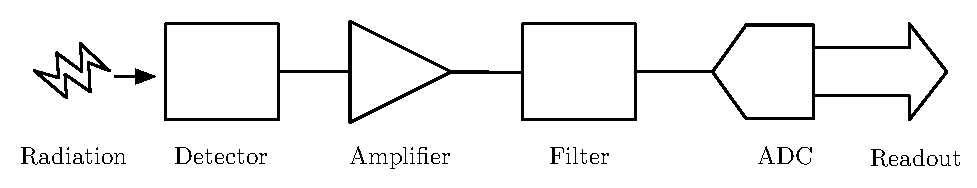
\includegraphics[width=5in]{./Figures/detector.eps}
	\caption[Diagram for a single channel circuit for particle physics experiments.]{Block diagram for a single channel, generic instrumentation circuit for particle physics experiments.}
	\label{fig:intint}
\end{figure}

The initial amplifier translates the input charge signal, coming from the detector electrodes, into an output voltage signal. Charge-to-voltage conversion is done by transferring the charge $Q_{in}$ from the nonlinear detector capacitance to a linear, known capacitor $C$. The output voltage is given by $V_{out} = Q_{in}/C$, with $C$ easily selectable and precisely tailorable. Fig.~\ref{fig:csa_post} depicts the most common preamplifier implementation, which consists of a voltage amplifier with a capacitor in a negative feedback configuration. The resulting circuit is a charge-sensitive amplifier (CSA), extensively studied in the literature \citep{Snoeys100,Asp100,deGeronimo500,oconnor100,Alvarez101}. The amplified signal includes noise from the detector and the CSA. Since the noise statistics are well modeled, they can be used to design a filter that maximizes the signal-to-noise ratio (SNR) at the detector front-end output. Usually the filter is an analog block, either time-invariant or time-varying, used to convert the voltage signal at the CSA output into a shaped voltage pulse. The pulse shape defines the weights of noise sources on the front-end output noise. Thus, a proper selection of the pulse shape is part of the solution to the SNR maximization problem. A memory acts as a buffer necessary to store data for a number of events before readout. For high-frequency pulse trains, analog memory is particularly well suited \citep{Kleinfelder100,Haller100}. Filtered signals can be quickly stored as charge in integrated capacitors, to be converted into digital signals by dedicated ADCs during the readout phase. Integration and feature size reduction has allowed the design of highly dense digital memory arrays. If a digital memory is used instead, ADCs are used to digitize the signal prior to storage, and conversion throughput per IC must be as high as the collision rate times the number of channels. 

\begin{figure}[!t]
	\centering
	\includegraphics[width=2in]{./Figures/csa_post}
	\caption{CSA using a voltage amplifier. Detector is modeled as a photodiode.}\label{fig:csa_post}
\end{figure}


\section{Noise minimization in circuits for particle physics instrumentation}
\subsection{Basic notions}
Noise, in the broadest sense, can be defined as any unwanted disturbance that obscures or interferes with a desired signal \citep{motchenbacher}. In electronics, noise is a random fluctuation that results from the physics of the devices and materials that make up the electrical system. It represents an important issue in the design of integrated circuits, since it determines the smallest signal level that can be processed on any real circuit. Noise generated by electronic devices, such as field-effect transistors and bipolar transistors, varies widely, as the operation of these devices involves several different physical processes, with many of them prone to spontaneous fluctuations. There are three sources of fundamental noise in MOSFETs \citep{gray101}: shot noise due to gate leakage current, thermal (for strong inversion operation) or shot (for weak inversion operation) noise in the channel, which is always white noise, and flicker or $1/f$ noise, also called pink noise. These noise sources have been extensively studied over the years, and several works about them can be found in the literature. References \citep{gray101,jindal101} are good starting points for introducing the reader into this subject.

As most times noise is assumed to be a stationary stochastic process, it is natural to study it in the frequency domain, where it is commonly expressed as a noise power spectral density. The integral of the noise power spectrum over the circuit bandwidth yields the total circuit noise power, and its square root is the standard deviation.% of either the noise voltage or noise current.

In an electronic circuit, composed by a number of electronic devices, there are several noise sources. To quantitatively compare the effect of these noise sources, each one of them can be referred to a common node of the circuit, typically the input node. Noise sources referred to the same circuit node are added up as follows:
\begin{equation}
\sigma^2_\textit{Total} = \sum_{i=1}^{N}\sigma^2_i + \sum_{i\neq j} c_{i,j} \cdot \sigma_i \cdot \sigma_j
\end{equation}
%\sigma^2_1 + \sigma^2_2 + 2\cdot c \cdot \sigma_1 \cdot \sigma_2
where $\sigma_i^2$ represents the noise power of source $i$, $N$ is the number of noise sources, and $c_{i,j}$ is the correlation coefficient between two noise sources.

By referring the noise sources to the input of the circuit, it is possible to make a fair comparison of noise performance among different circuits with common application, and set the total input-referred noise as a figure of merit. In a linear circuit, the total \mbox{input-referred} noise can be represented by a combination of a series voltage noise source ($V_n^2$) and a parallel current noise source ($I_n^2$), as shown in Fig.~\ref{fig:noise_cir}. If the driving signal is a low-impedance voltage source, the voltage noise is dominant and the current noise can be neglected, whereas if the signal source is a high-impedance current source, the voltage noise can be neglected, as current noise accounts for all the circuit noise. In circuits with a non-ideal load line, both noise sources must be considered.

\begin{figure}[!t]
	\centering
	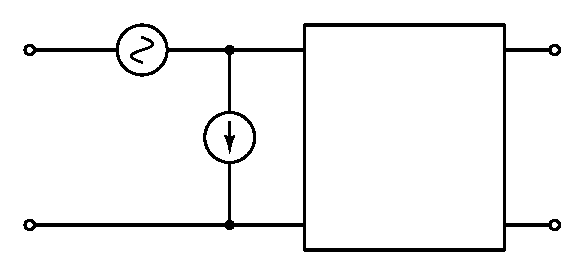
\includegraphics[width=3.2in]{./Figures/noise_cir}
	\caption[Linear circuit with internal noise sources referred to the input port.]{Equivalent representation of a linear circuit internal noise sources referred to the input port.}\label{fig:noise_cir}
\end{figure}

\subsection{Noise minimization in particle physics instrumentation systems}
In general, on any signal processing system, noise minimization is carried out through a careful design of the first processing stages, which for particle physics experiments corresponds to the detector front-end circuit, and specifically, the detector electrodes, the CSA and the \mbox{pulse-shaper}. Understanding and designing for low noise has been one of the main concerns in modern particle physics instrumentation. Any survey on this topic starts with a work published in 1968 \citep{radeka104}, where important concepts of pulse shaping for particle physics experiments were described as well as introduced. Among these is the weighting function (WF) concept, a time-domain representation of the total integrated noise, a useful tool to calculate the noise of a typical detector front-end circuit, which is still in use nowadays. 

In 1972, a design-oriented time-domain analysis based on the WF concept was published \citep{goulding101}. In this work it was demonstrated that, assuming only white noise, all the noise sources in a detector front-end circuit can be reduced to two noise sources at the input node: a parallel noise source and a series noise source. Integration of each component in frequency yields two noise coefficients that make it possible to characterize the noise-filtering capabilities of a pulse shaper.

In 1988, results from previous works on noise were summarized in one of the most influential papers in low-noise techniques for particle physics instrumentation \citep{radeka101}. The formalization and stringency of this work guided the subsequent work on the field.

Study of flicker noise in particle physics electronics was introduced in \citep{lutz101}. Before this work, flicker noise was almost never considered in the design for particle physics electronics. In 1990, the problem of finding the optimum WF for particle physics electronics, including flicker noise in the analysis, was published \citep{gatti104}. The same year, an excellent derivation of noise for particle physics front-end electronics, including thermal, flicker and shot noise sources was presented \citep{sansen101}.

In \citep{gadomski101}, the deconvolution method for pulse-shaping was presented. Major innovations of this work come from the use of switched-capacitor filters for \mbox{pulse-processing} purposes and the introduction of the concept of \mbox{discrete-time} \mbox{pulse-shaping}.

In \citep{pullia104}, for the first time the flicker noise is analyzed in the time domain. A generalization of this work was presented in \citep{pullia102}, allowing time-domain simulations of almost all kind of noise sources.  This work represents a powerful tool for computer-aided filter design.

Finally, excellent books on particle physics instrumentation systems have been published \citep{radeka201}, compiling and explaining the results from many papers in the field.


\section{Thesis content}
Chapter 2 starts with an introduction to the project that prompts the work of this thesis, the design and implementation of a second iteration of the Bean, an instrumentation application-specific integrated circuit (ASIC) which forms part of the proposal for the ILC. It is followed by an overview of the motivations that led to the development of a new mathematical framework for noise analysis in discrete-time filters, alongside with the presentation of the requirements for a filter intended to take full advantage of this framework. Chapter 3 presents the complete formulation of this noise analysis, including examples and applications for optimal filter computation. In Chapter 4 , the design and implementation of a filter for arbitrary weighting function synthesis are presented. Chapter 5 shows the results that contribute to the ongoing project, functionality verifications of the designed filter and the implementation of an early prototype of the Bean V2, with the filter as one of its core building blocks. Finally, Chapter 6 summarizes the results and contributions of this work, and presents ideas for future research.